\documentclass[12pt]{article}
\usepackage[margin=1in]{geometry} 
\usepackage{amsmath,amsthm,amssymb,amsfonts, graphicx}

\newtheorem{theorem}{Theorem}[section]
\newtheorem{corollary}{Corollary}[theorem]
\newtheorem{lemma}[theorem]{Lemma}
 
\renewcommand{\thefootnote}{\fnsymbol{footnote}}
\newcommand{\N}{\mathbb{N}}
\newcommand{\Z}{\mathbb{Z}}
 
\newenvironment{problem}[2][Problem]{\begin{trivlist}
\item[\hskip \labelsep {\bfseries #1}\hskip \labelsep {\bfseries #2.}]}{\end{trivlist}}
 
\begin{document}
 
%\renewcommand{\qedsymbol}{\filledbox}
%Good resources for looking up how to do stuff:
%Binary operators: http://www.access2science.com/latex/Binary.html
%General help: http://en.wikibooks.org/wiki/LaTeX/Mathematics
 
\title{Homework 10}
\author{Tanner Kvarfordt - A02052217}
\maketitle

\noindent Define $\Gamma$ to be the graph with vertex set the $2$-sets of $\{1,2,3,4,5\}$ and vertices adjacent if and only if they are disjoint. the following lemmas apply. \\

\noindent\textbf{Lemma 4.18.1} \textit{The degree of every vertex of $\Gamma$ is $4$ and $\Gamma$ has $15$ edges.} \\

\noindent A \textbf{cycle} of length $k$ in a (di)graph $G$ is a sequence of vertices $(v_1,v_2,...v_k,v_1)$ where $v_iv_{i+1} \in E(G)((v_i,v_{i+1})\in A(G))$ for $1 \leq i \leq k-1$ and $v_kv_1 \in E(G)((v_k,v_1)\in A(G))$. \\

\noindent\textbf{Lemma 4.18.2} \textit{The graph $\Gamma$ has no cycles of length $k$ for $k=2,3,4$}.

\begin{problem}{1}
Two graphs $G$ and $H$ are homeomorphic if there exists a graph $\Gamma$ such that each of $G$ and $H$ can be obtained from subdivisions of $\Gamma$. Please sort the trees on 8 vertices into homeomorphism classes.
\end{problem}
 
\begin{proof}[Answer]
All trees on 8 vertices are drawn in the following pictures, each with the corresponding number of their homeomorphism class\footnote{These "homeomorphism numbers" mean nothing, they are simply a method by which to distinguish homeomorphism classes.} in the upper right hand corner and the corresponding $\Gamma$ in the bottom left corner. These trees were obtained by conditioning on diameter (beginning at 8 and continuing down to 4) and drawing each distinct possibility on that diameter so that as many possibilities as possible were created without any isomorphism occurring. \\
\begin{center}
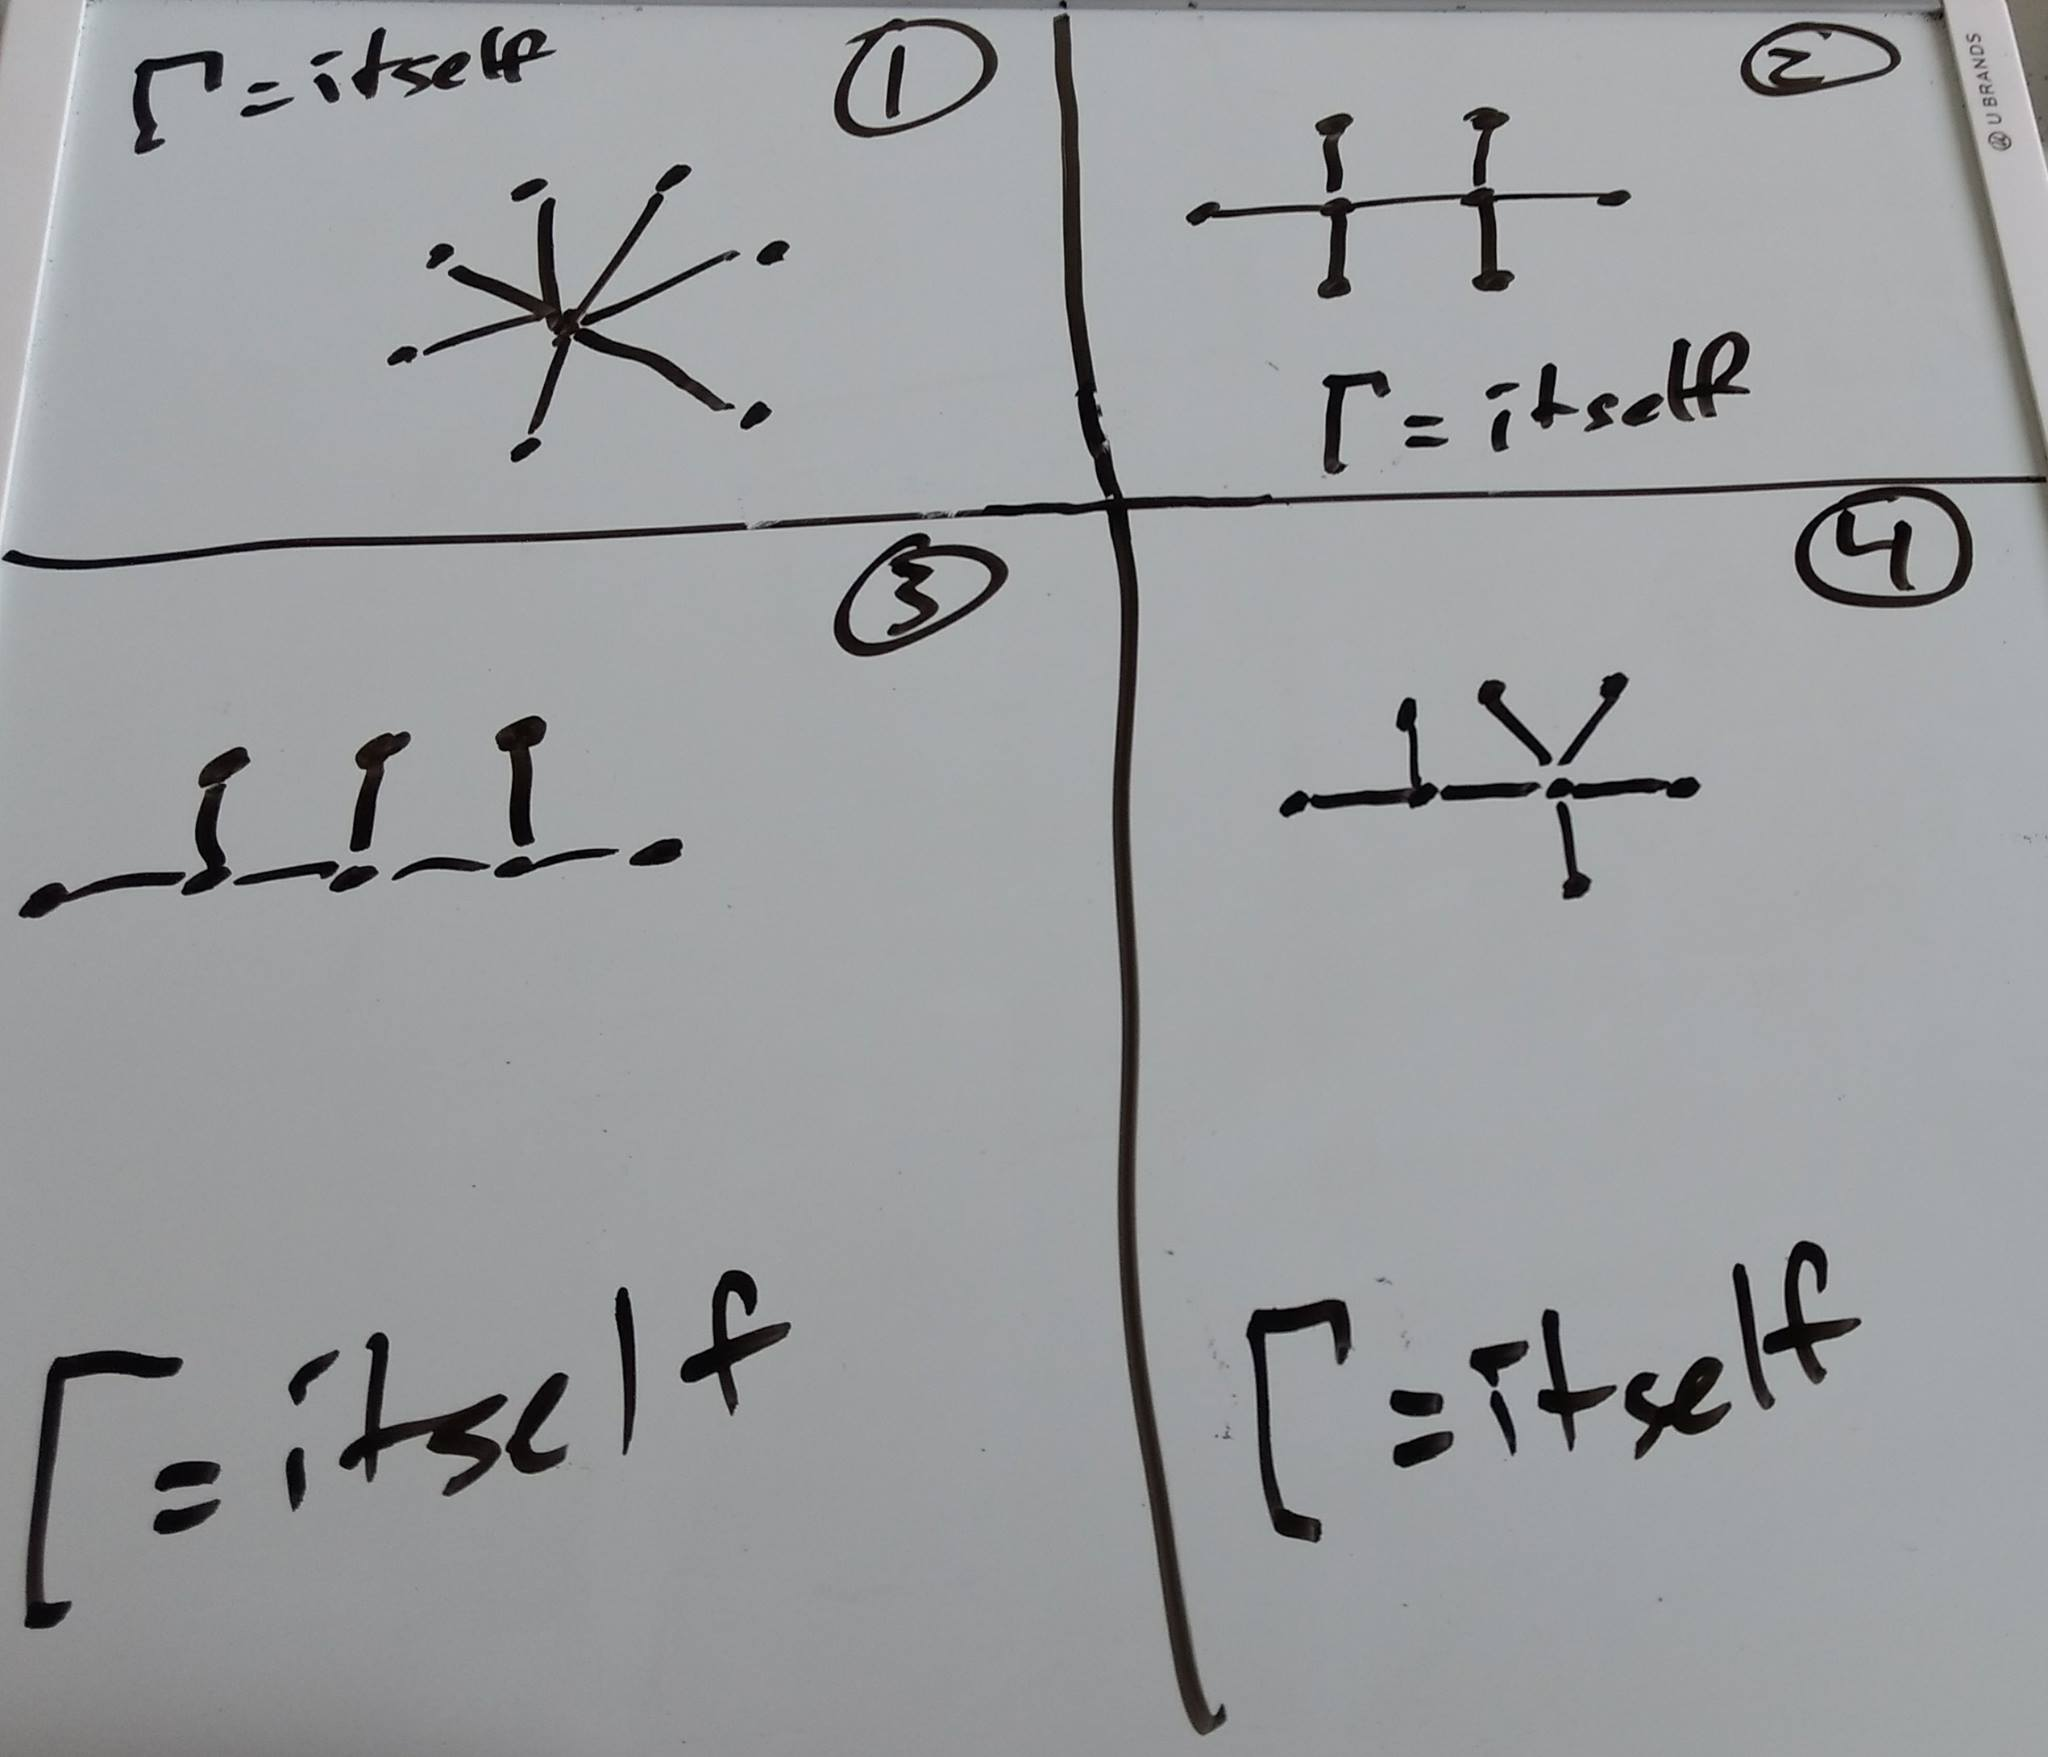
\includegraphics[scale=0.07]{1_4.jpg}
\hspace{0.05in}
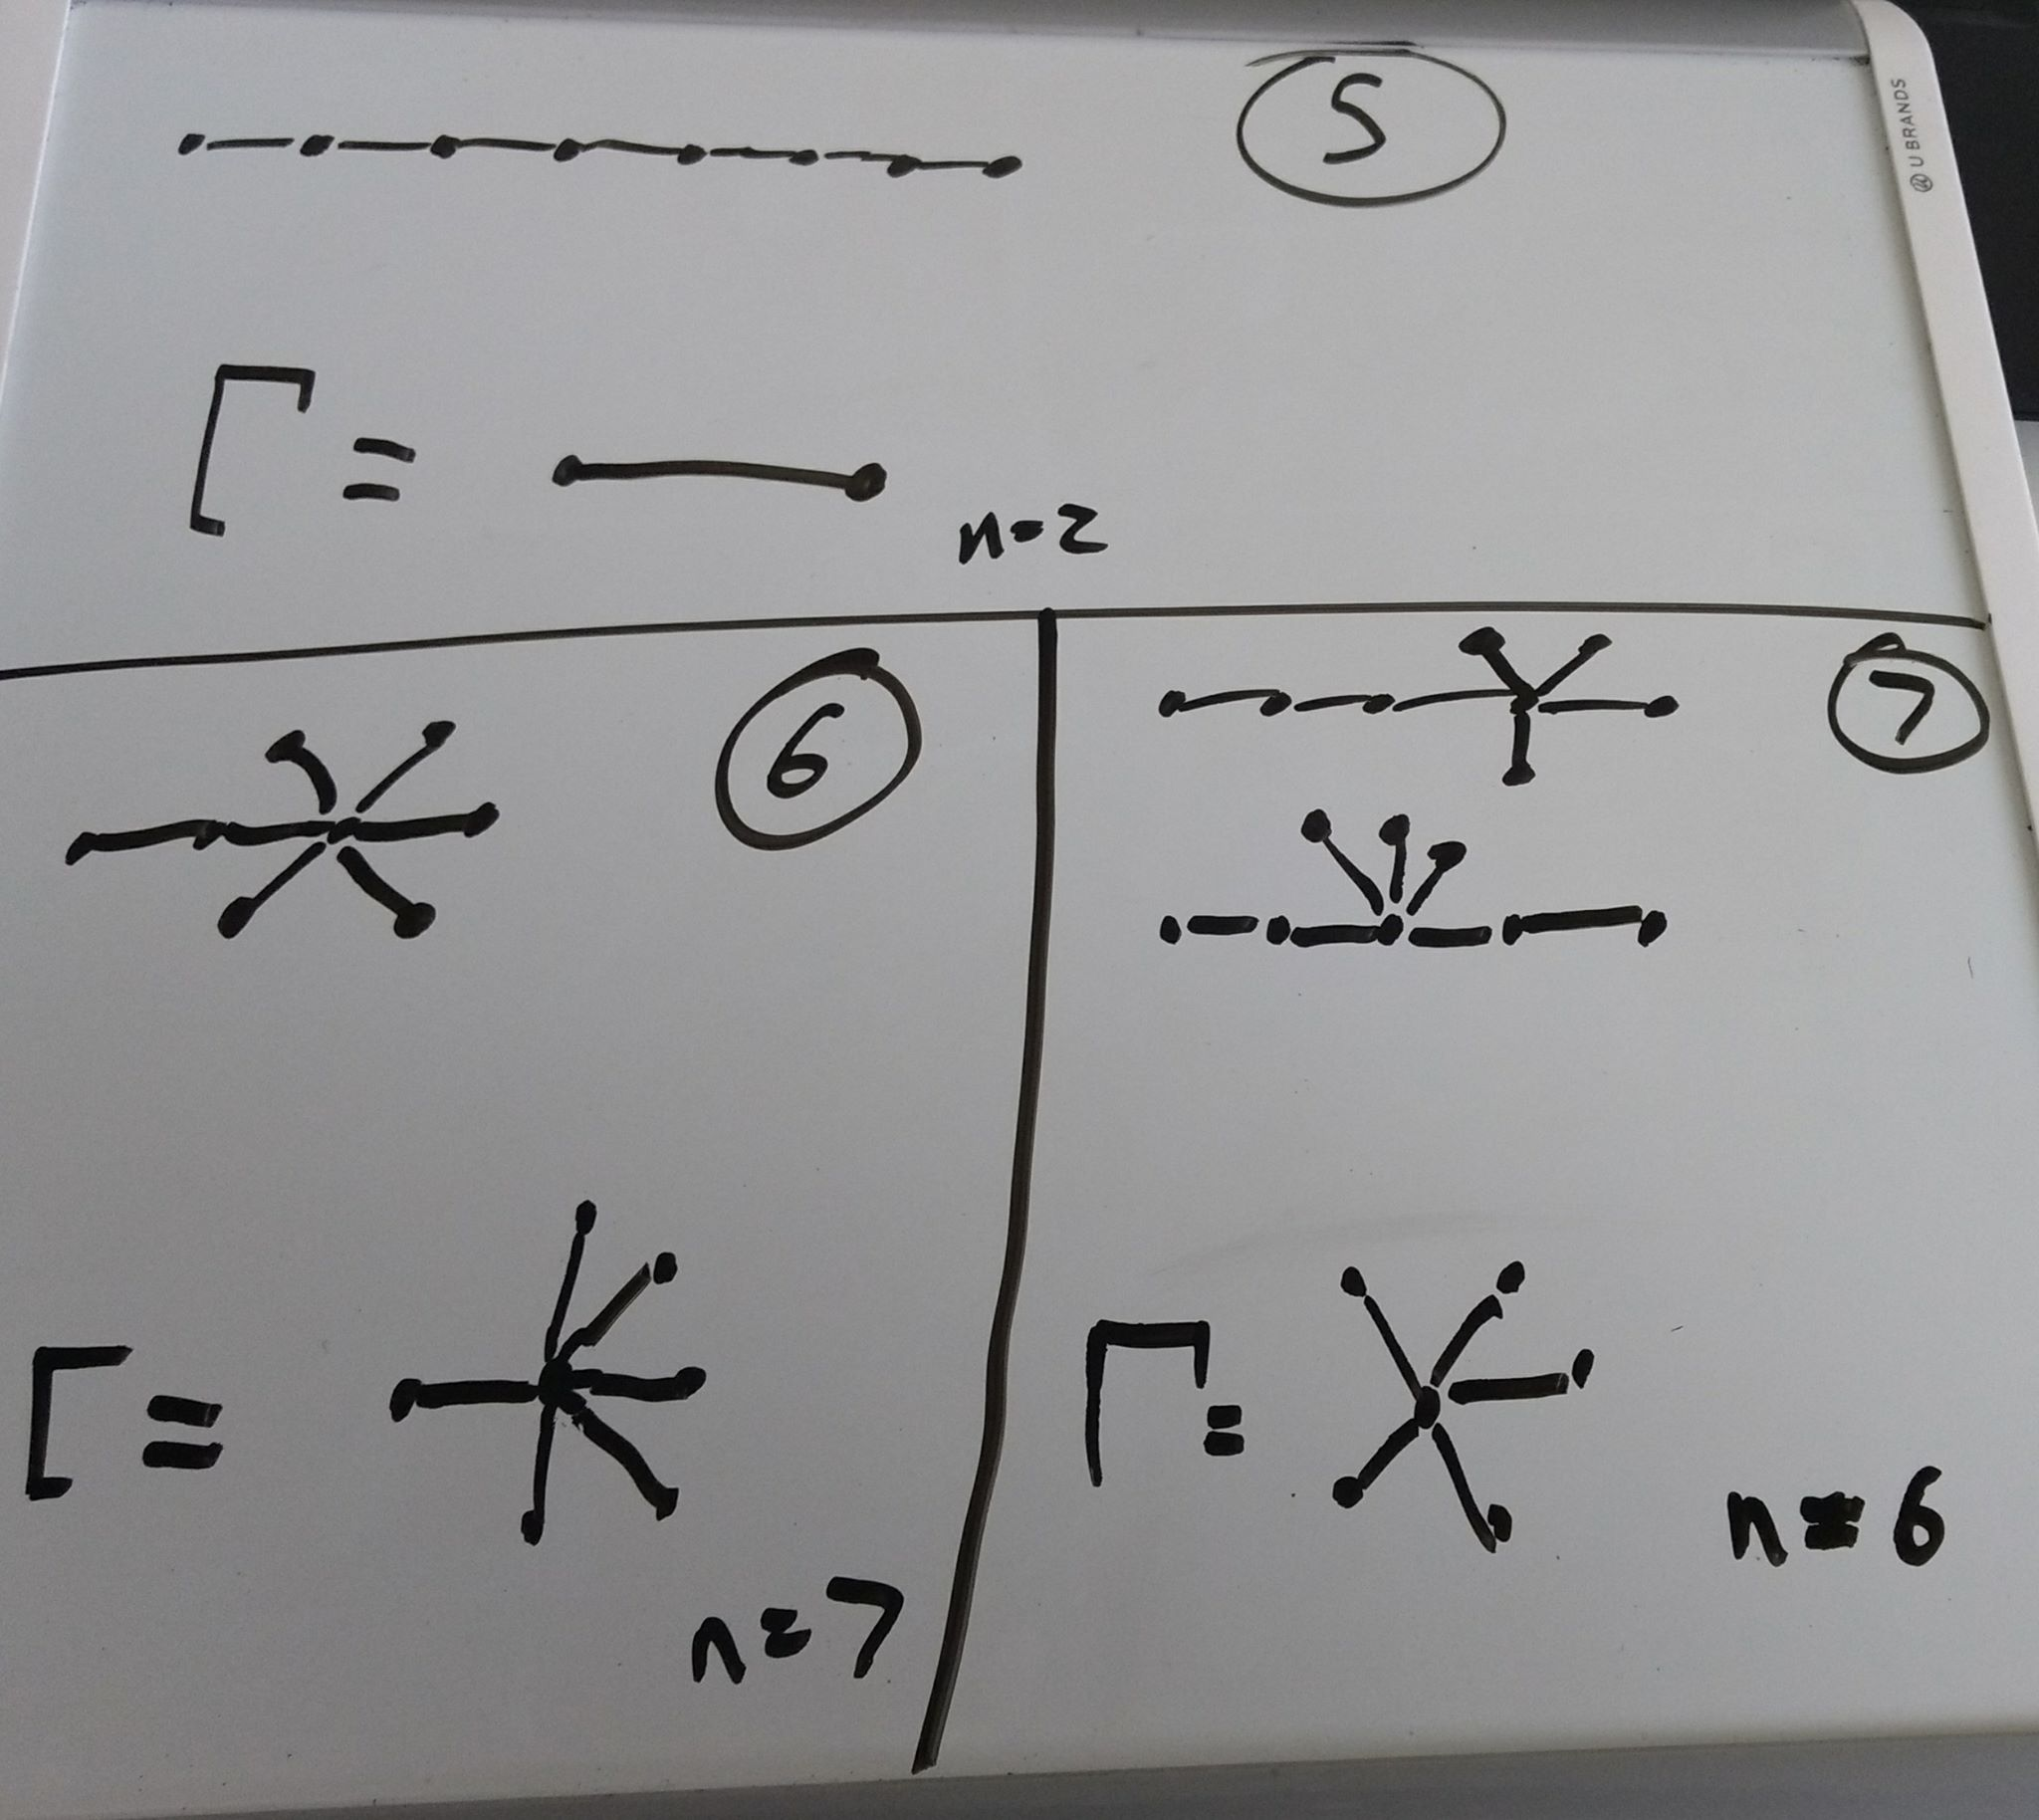
\includegraphics[scale=0.07]{5_7.jpg}
\hspace{0.05in}
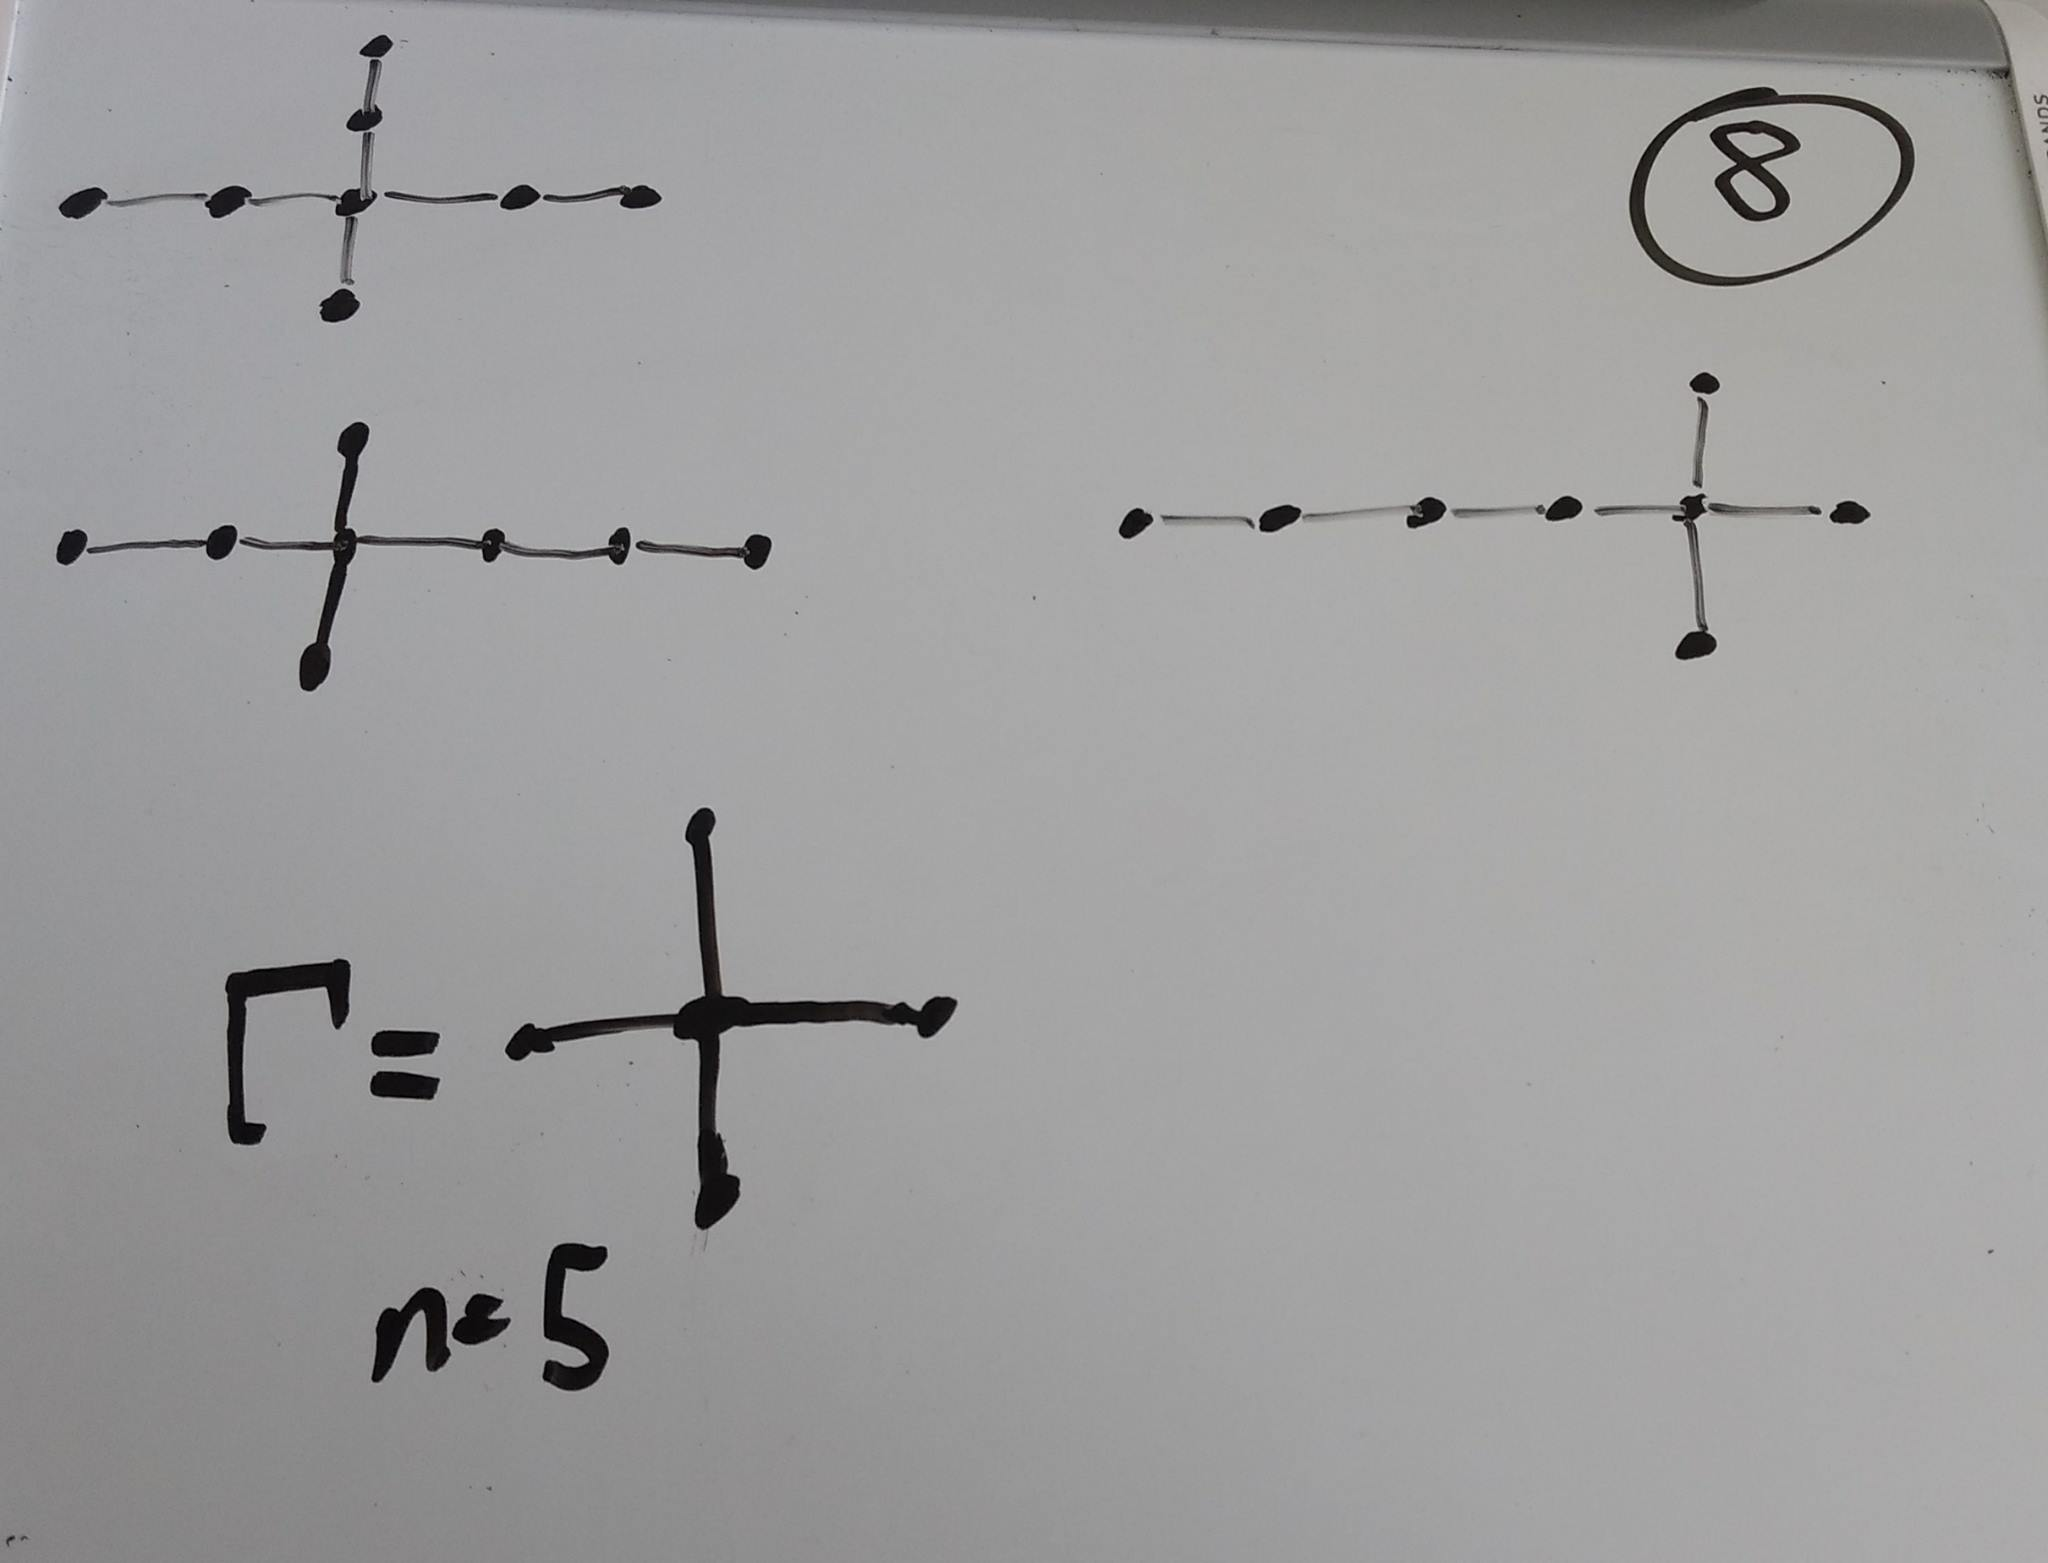
\includegraphics[scale=0.07]{8.jpg}
\end{center}
\begin{center}
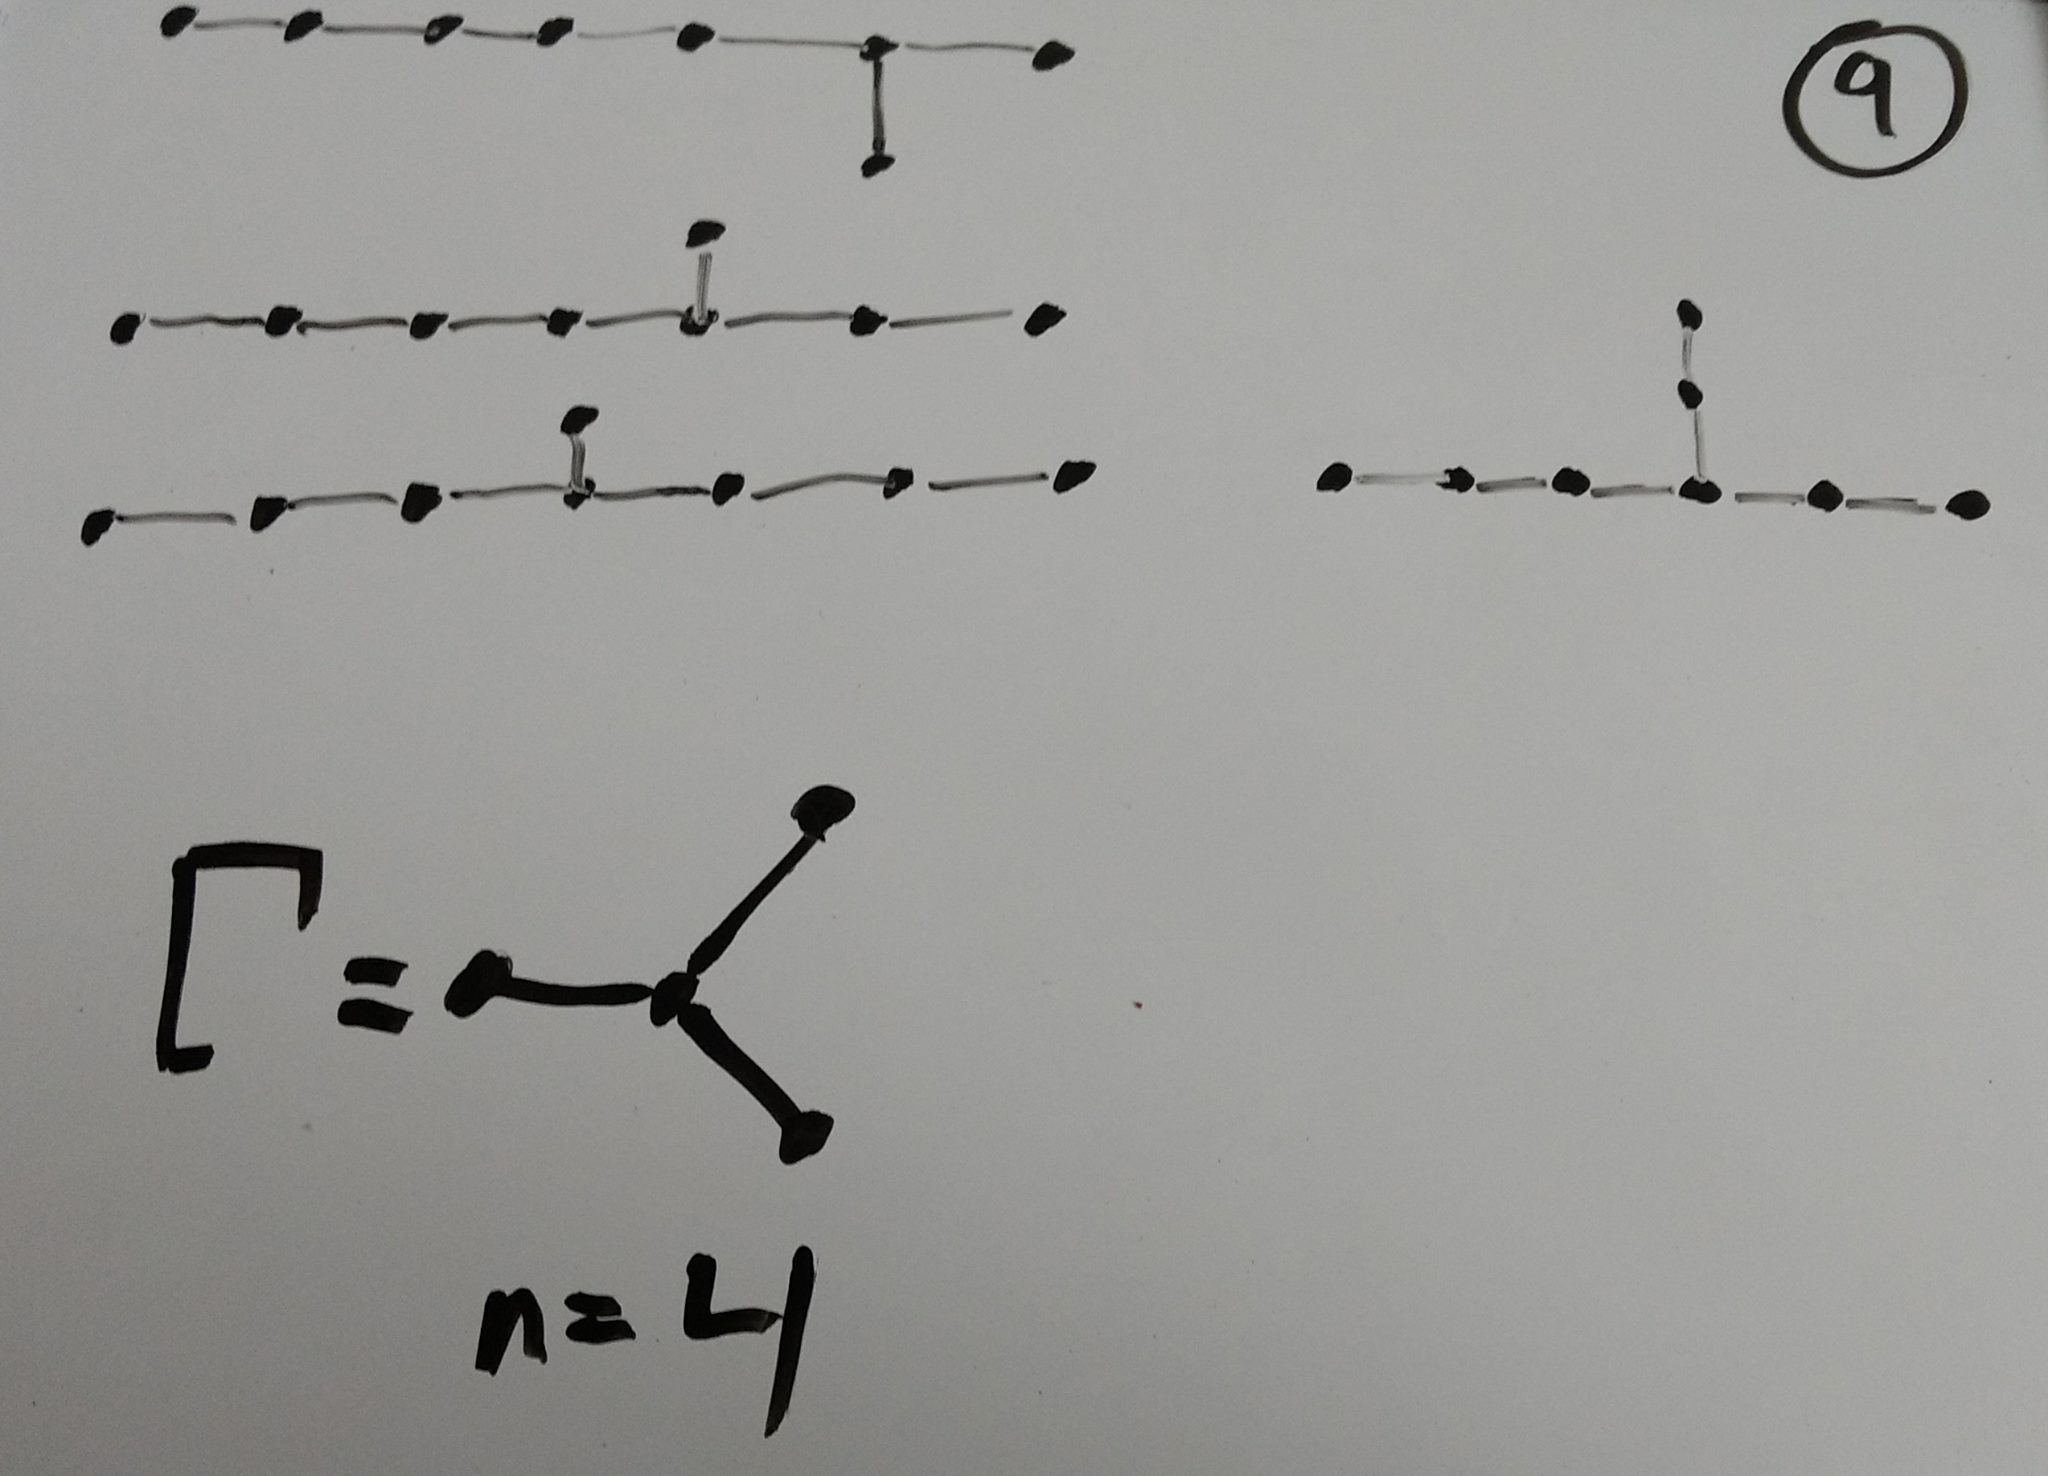
\includegraphics[scale=0.07]{9.jpg}
\hspace{0.05in}
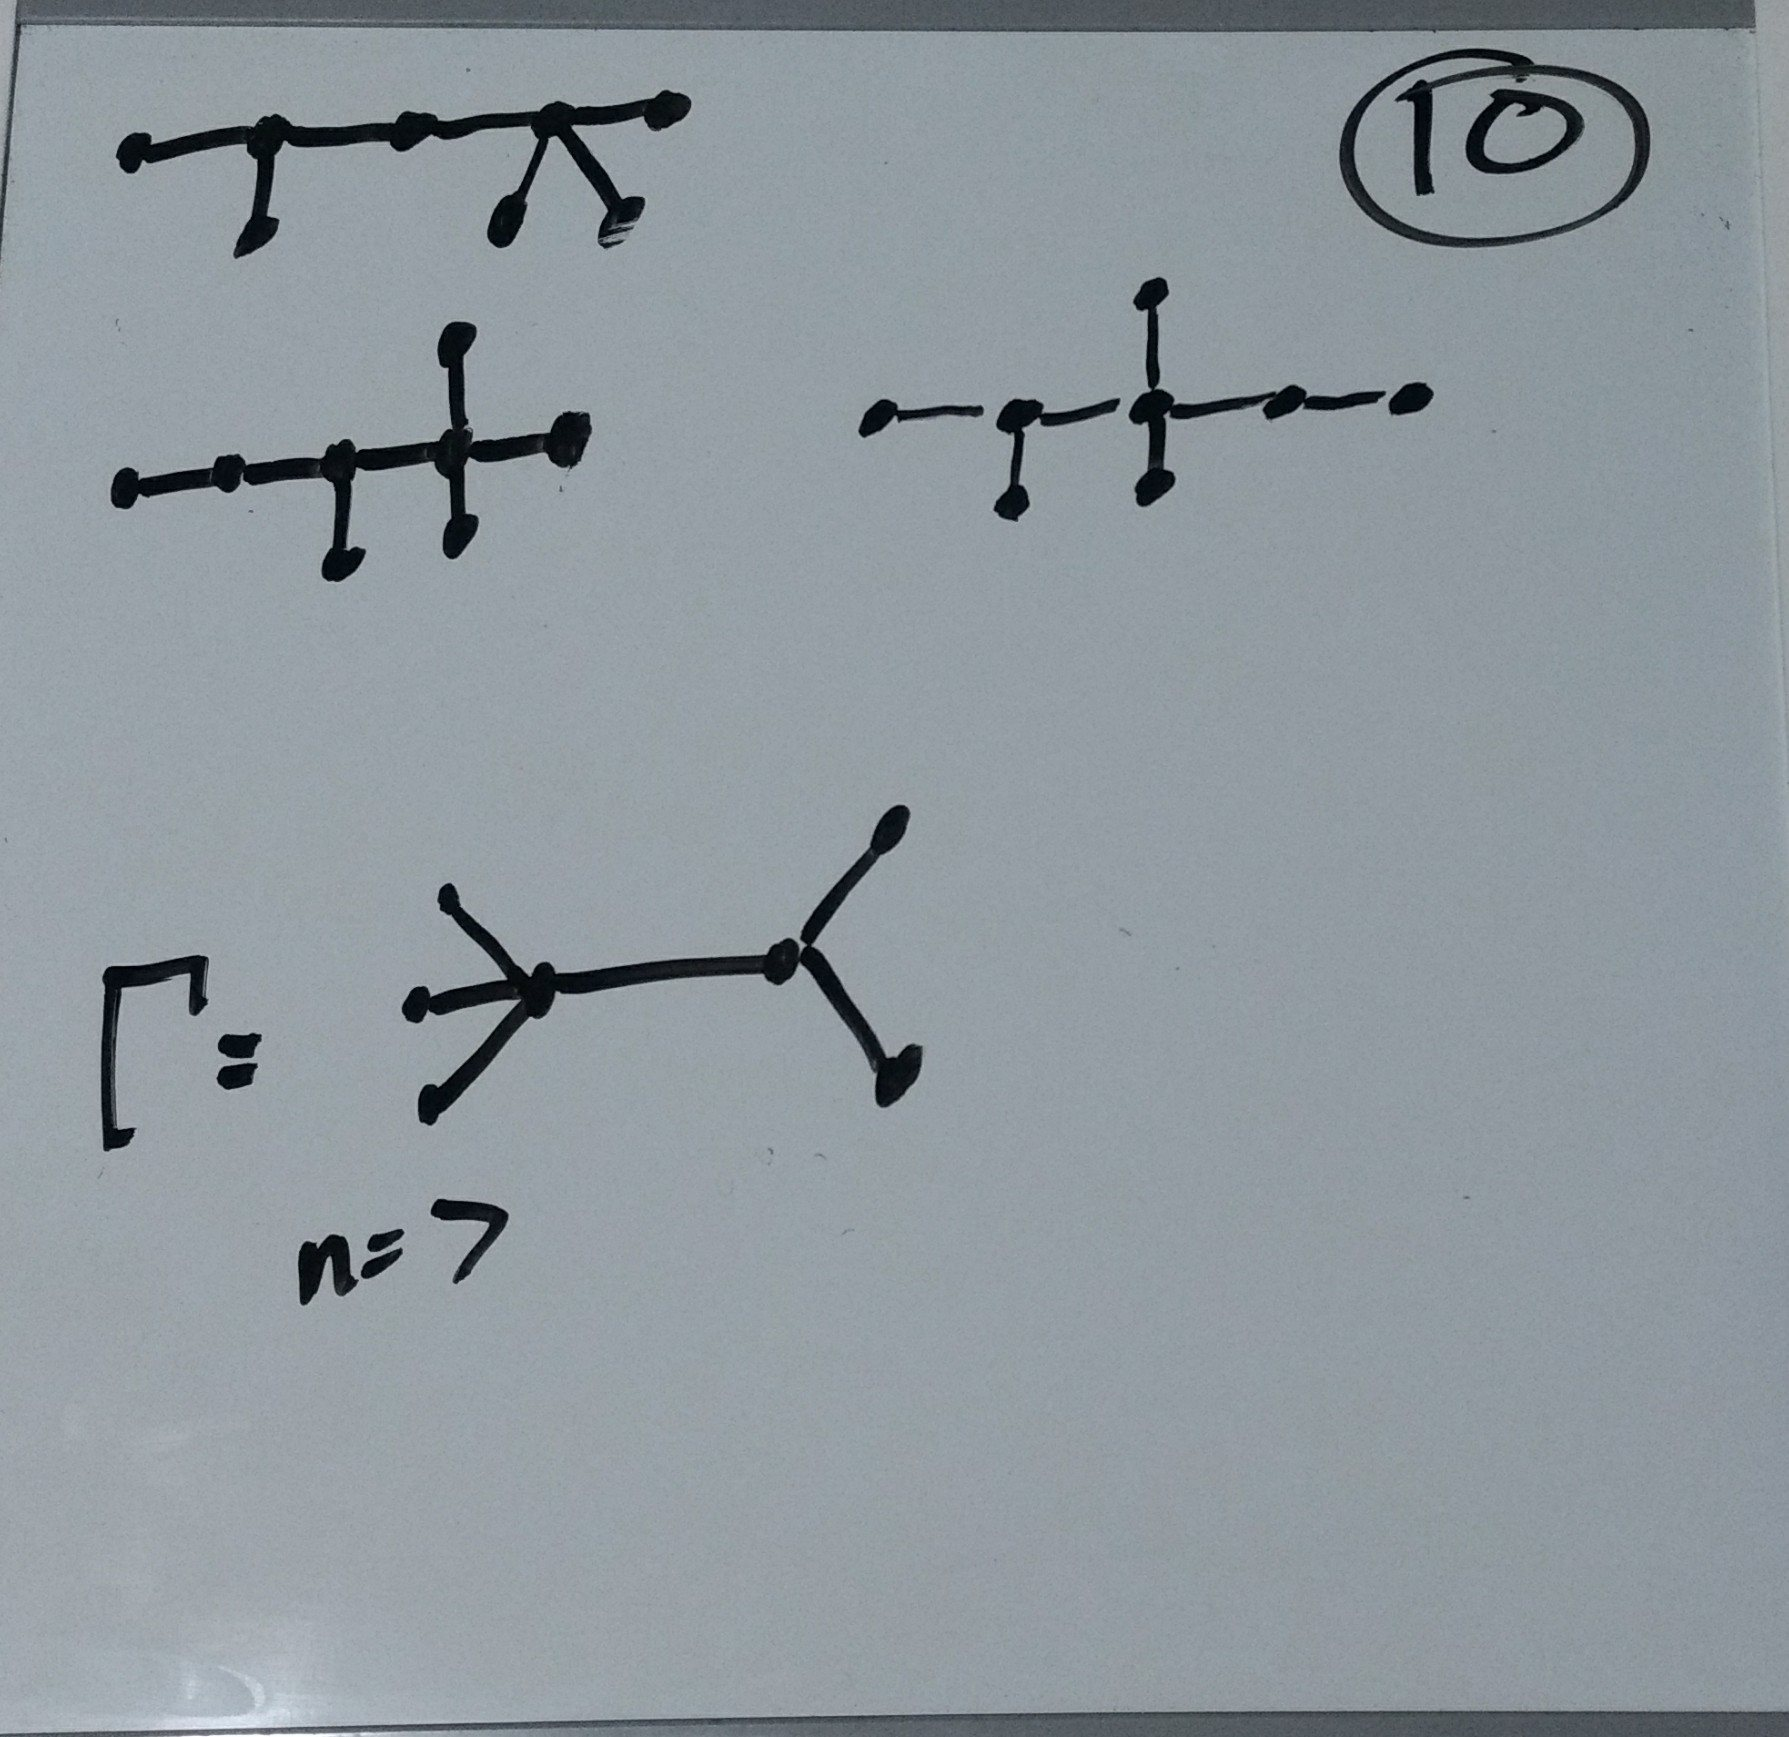
\includegraphics[scale=0.07]{10.jpg}
\hspace{0.05in}
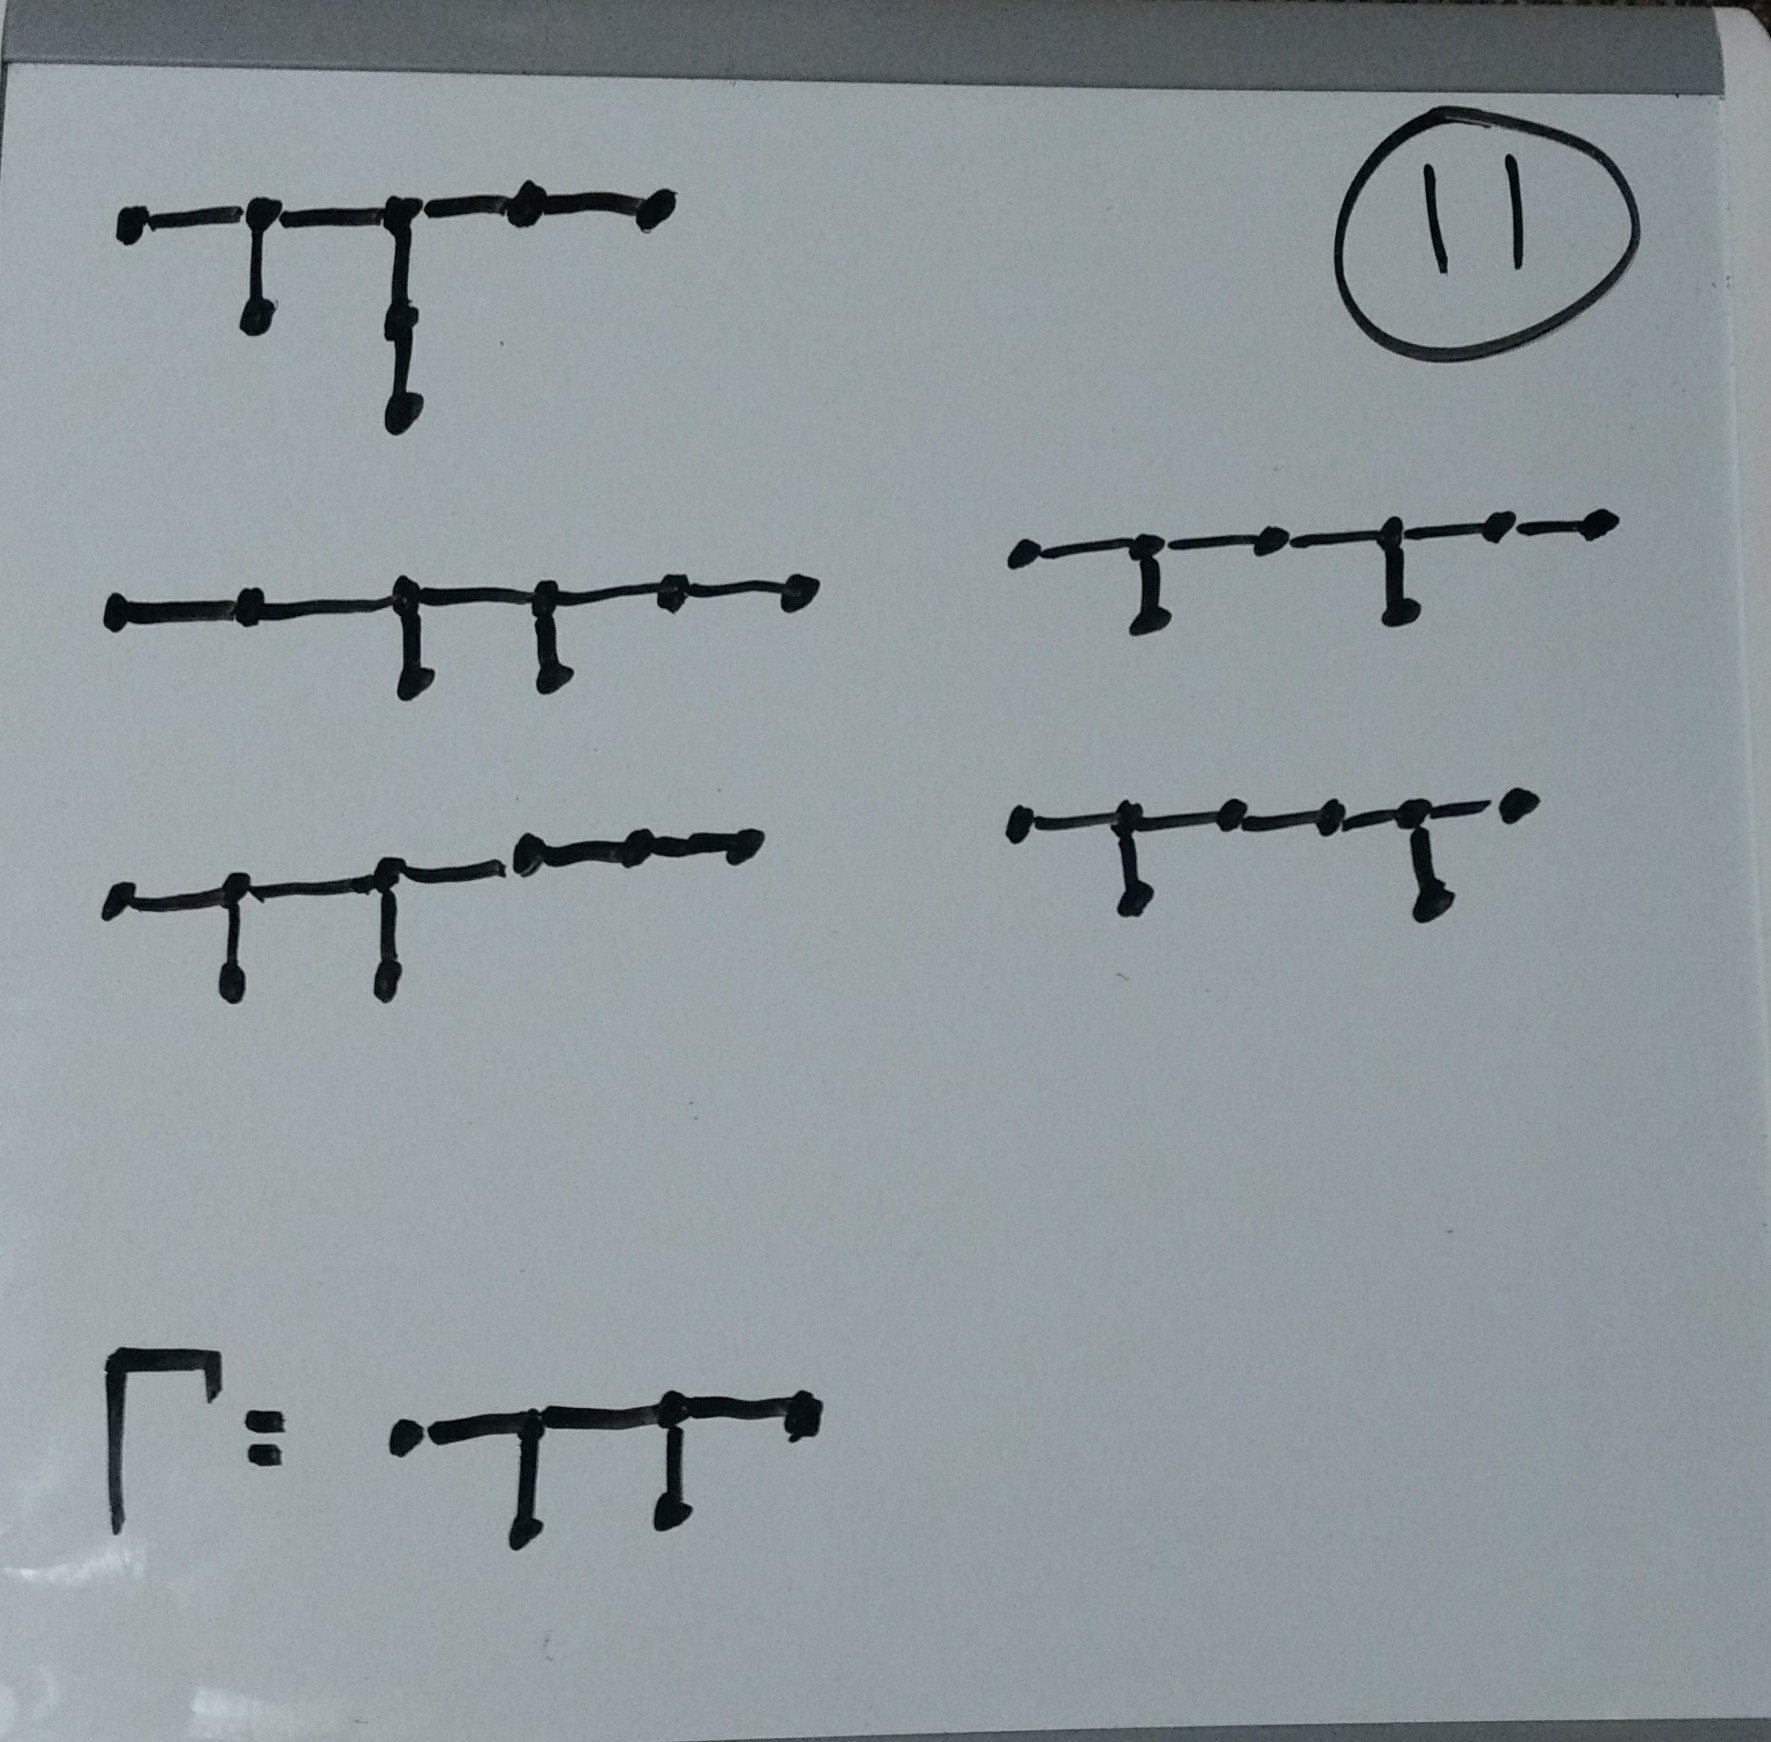
\includegraphics[scale=0.07]{11.jpg}
\end{center}
\end{proof}

\begin{problem}{2}
Please prove the following graph $\Gamma$ is not planar using $(1)$ Kuratowski's Theorem and $(2)$ using Euler's formula. The graph $\Gamma$ has vertex set the set of all 2-element subsets of $\{1,2,3,4,5\}$ and vertices adjacent if and only if they are disjoint.
\end{problem}
 
\begin{proof}[Proof via Euler's Formula]
This will be a proof by contradiction. Recall Euler's Formula for a planar graph:
\[n-e+f=2\]\nonumber
Where $f$ is the number of 2-D faces in the planar graph, $n$ is the number of vertices, and $e$ is number of edges. So for $\Gamma$, we can plug in $e$ and $n$ to solve for $f$, giving $f=7$. \\
Now consider $l(F):=$ the number of edges that border a particular face $F$ in any given planar graph, and the set $H$ of all faces in that planar graph, so $\sum_{F \in H}l(F)=2e$. For $\Gamma$, then supposedly $\sum_{F \in H}l(F)=30$. However, according to lemma 4.18.2, $\Gamma$ cannot have a cycle of length less than $5$\footnote{Yes, I know I haven't proven that there is a cycle of length 5 in $\Gamma$, but I contend that this is an irrelevant detail since the important thing to note here is that there are certainly no cycles \textbf{less} than $5$ in length.}, and therefore $\sum_{F \in H}l(F)\geq5f$, where $5f=35$ according to Euler's formula. Clearly, $35 \neq 30$, therefore $\Gamma$ cannot be planar.
\end{proof}

\begin{proof}[Proof via Kuratowski's Theorem]
$\Gamma$ is drawn below. 
\begin{center}
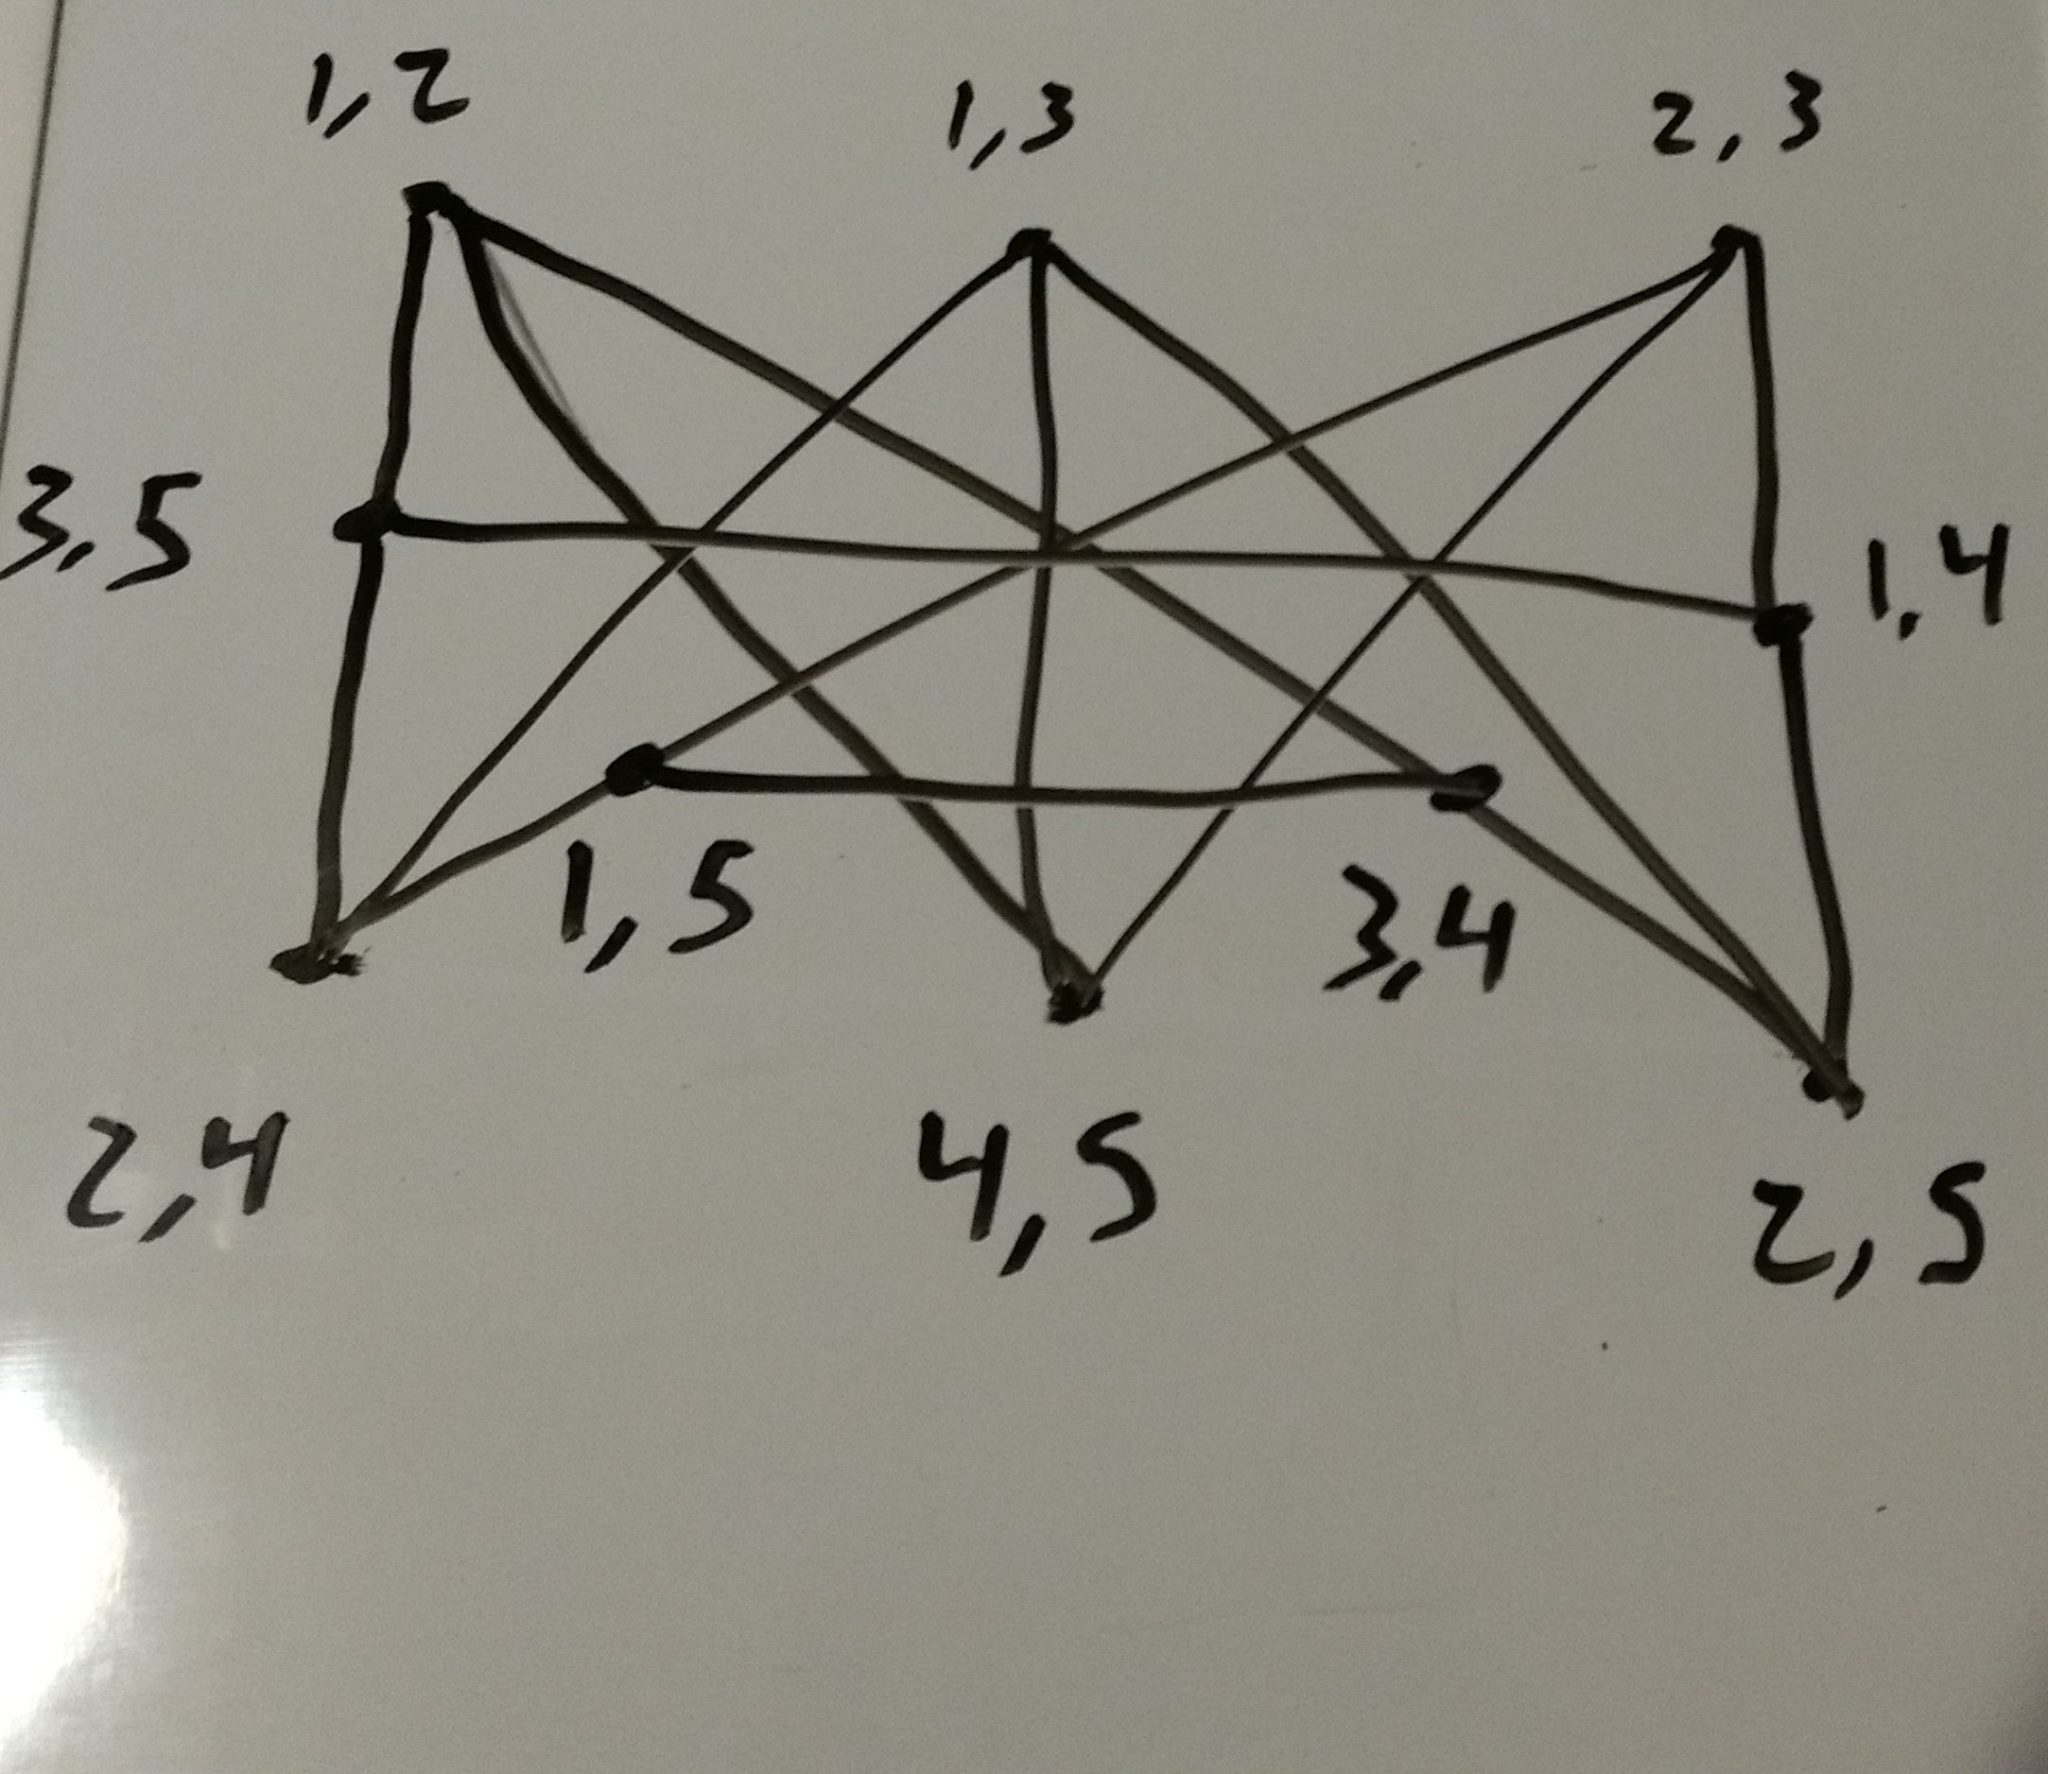
\includegraphics[scale=0.1]{Gamma.jpg}
\end{center}
Disregard, for a moment, the edge between vertex $3,5$ and $1,4$, as well as the edge between $1,5$ and $3,4$. This subgraph\footnote{Subgraph $:=$ A subgraph of a graph G is another graph formed from a subset of the vertices and edges of G. The vertex subset must include all endpoints of the edge subset, but may also include additional vertices. Credit for this lovely definition goes to Wikipedia} is clearly homeomorphic to $K_{3,3}$. Kuratowski's Theorem states that a graph is planar if and only if it and all of its subgraphs are not homeomorphic to $K_{3,3}$. Since $\Gamma$ has a subgraph homeomorphic to $K_{3,3}$, it therefore cannot be planar.
\end{proof}

\begin{problem}{3}
Use Graph Theory to model and describe the following problem's solution. Suppose $C=\{c_1,c_2,...,c_n\}$ is a collection of chemicals which must be stored very carefully at very specific temperatures. For each $c_i \in C$, you know the lowest temperature at which it can be stored, call it $l_i$, and the highest temperature at which it can be stored, call it $h_i$. Here's the problem: Determine the smallest number of temperature-controlled storage units into which the chemicals can be stored.
\end{problem}
 
\begin{proof}[Answer]
Let $G := ($family of temperature intervals for $c_1$ through $c_n$, $E)$, such that $V(G)=\{c_1,c_2,...,c_n\}$ where $c_i,c_j\in V(G)$ and $c_ic_j \in E(G) \implies (l_i,h_i) \cap (l_jh_j) \neq \varnothing$. Consider a temperature-controlled storage unit. if there is a temperature, $t$, for two chemicals, $c_i,c_j\in C$ where $l_i \leq t \leq h_i$ and $l_j \leq t \leq h_j$, then $c_i$ and $c_j$ can be stored together. Now consider a vertex clique in $G$. By the definition of $G$ above, two chemicals (vertices) have an edge between them if the two chemicals have storage temperature intervals that are indifferent to each other, essentially, if there is a temperature $t$ that exists as defined. Therefore the vertex-clique cover number, $\theta_v(G)$, gives the minimum number of storage units into which the chemicals can be stored.
\end{proof}

\end{document}